\section{Numerical results}
\label{sec:numerical}

\subsection{Comparison with methods based on finite differences}
\label{ssec:fd}

We first compare the performance of \gls{newuoa} using \gls{pdfo} with \gls{bfgs} and \gls{cg}, two gradient-based solvers provided by SciPy~\cite{Virtanen_Etal_2020}.
When no derivatives are provided, they use forward finite-difference to approximate gradients, with the difference parameter~$h = \sqrt{u}$, where~$u$ is the unit roundoff.
We perform the comparison on the unconstrained problems of dimensions at most~$50$ from the CUTEst library~\cite{Gould_Orban_Toint_2015}.
In this comparison, we invoke \gls{newuoa} via the \gls{pdfo} package under the default settings.
In particular, the initial trust-region radius is~$1$, the final trust-region radius is~$10^{-6}$, and the number of interpolation points is~$2n + 1$, with~$n$ being the dimension of the problem being solved.
\Gls{bfgs} and \gls{cg} are called with the default configurations in SciPy.
For each testing problem, the starting point is set to the one provided by CUTEst, and the maximal number of function evaluations is set to~$500$ times the number of variables.

We conduct two experiments as follows.
\begin{enumerate}
    \item The first experiment is made without modifying the problems.
    The optimal value~$\obj_{\ast}$ of a given problem is considered to be the least value reached by all solvers, and an execution is convergent up to a tolerance~$\tau \ge 0$ whenever
    \begin{equation}
        \label{eq:cvt}
        \obj(\iter[0]) - \obj(\iter) \ge (1 - \tau) [\obj(\iter[0]) - \obj_{\ast}].
    \end{equation}
    \item The second experiment is a noisy variation of the previous one.
    Let~$\sigma > 0$ be the noise level.
    For each problem, the objective function is evaluated by
    \begin{equation}
        \label{eq:noisy-obj}
        \tilde{\obj}(\iter[]) \eqdef [1 + \epsilon(\iter[])] \obj(\iter[]),
    \end{equation}
    where~$\epsilon(\iter[]) \sim N(0, \sigma^2)$.
    Each problem is solved ten times with each solver.
    In the convergence test~\eqref{eq:cvt},~$\obj_{\ast}$ is either the least value of~$\obj$ obtained by all solvers during these ten runs, or the value obtained in the previous noise-free experiment, whichever is smaller.
    Note that the convergence test~\eqref{eq:cvt} uses the values of~$\obj$ and not those of~$\tilde{\obj}$.
    This means that we evaluate the solvers according to the true objective function, even though the solvers can access only the noisy values produced by~\eqref{eq:noisy-obj}.
\end{enumerate}

The performance profiles~\cite{Dolan_More_2002,More_Wild_2009} of these experiments are provided in Figures~\ref{fig:ppu-fdiff-plain}--\ref{fig:ppu-fdiff-noisy-6}.
Broadly speaking, a performance profile plots the proportion of problems solved with respect to the number of function evaluations required to achieve convergence, in a logarithmic scale.

\begin{figure}[ht]
    \begin{subfigure}{.48\textwidth}
        \centering
        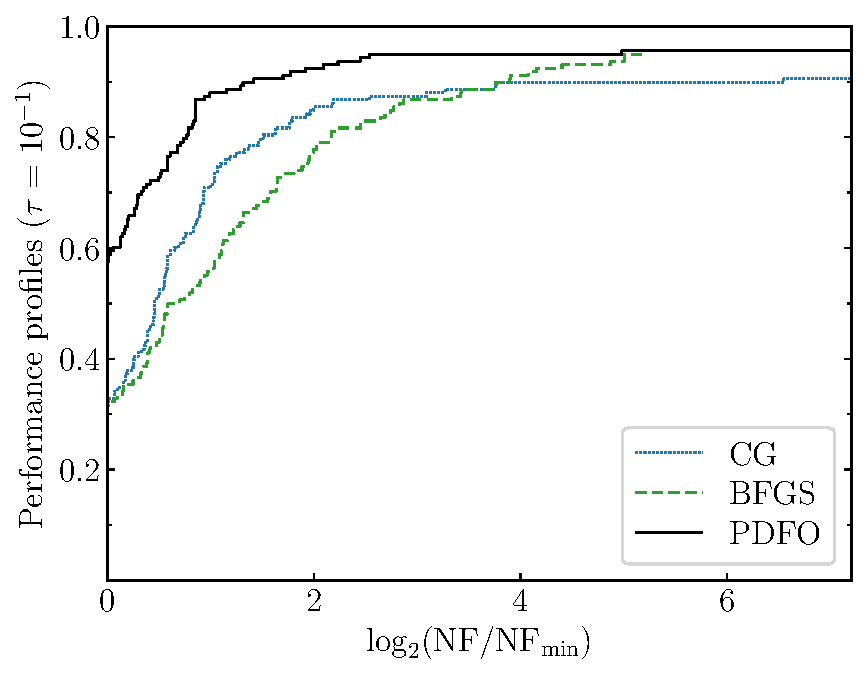
\includegraphics[width=\textwidth]{perf-plain-bfgs_cg_pdfo-50.pdf}
        \caption{Noise-free experiment}
        \label{fig:ppu-fdiff-plain}
    \end{subfigure}
    \hfill
    \begin{subfigure}{.48\textwidth}
        \centering
        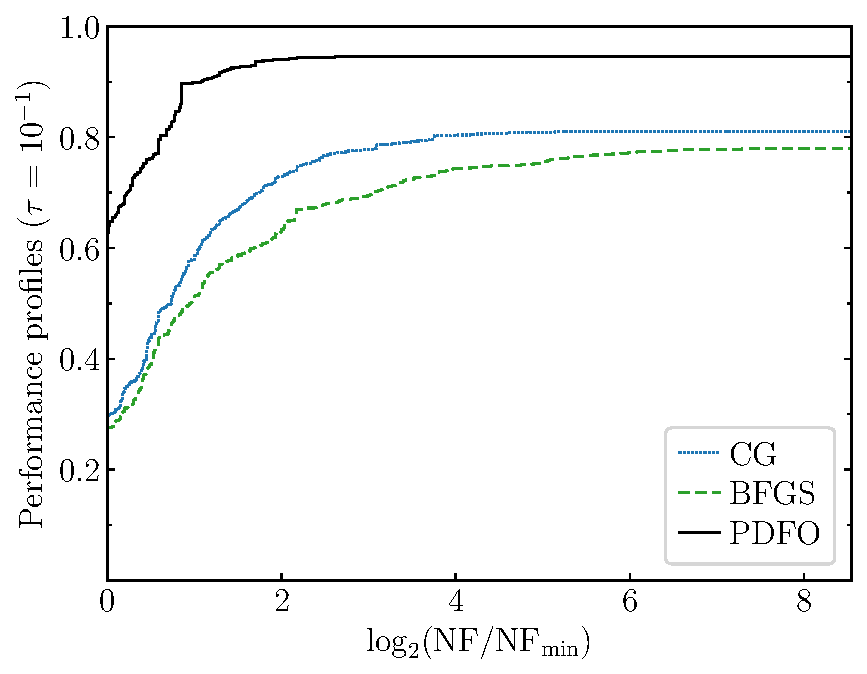
\includegraphics[width=\textwidth]{perf-noisy-bfgs_cg_pdfo-50-10.pdf}
        \caption{Noisy experiment with~$\sigma = 10^{-10}$}
    \end{subfigure}
    \begin{subfigure}{.48\textwidth}
        \centering
        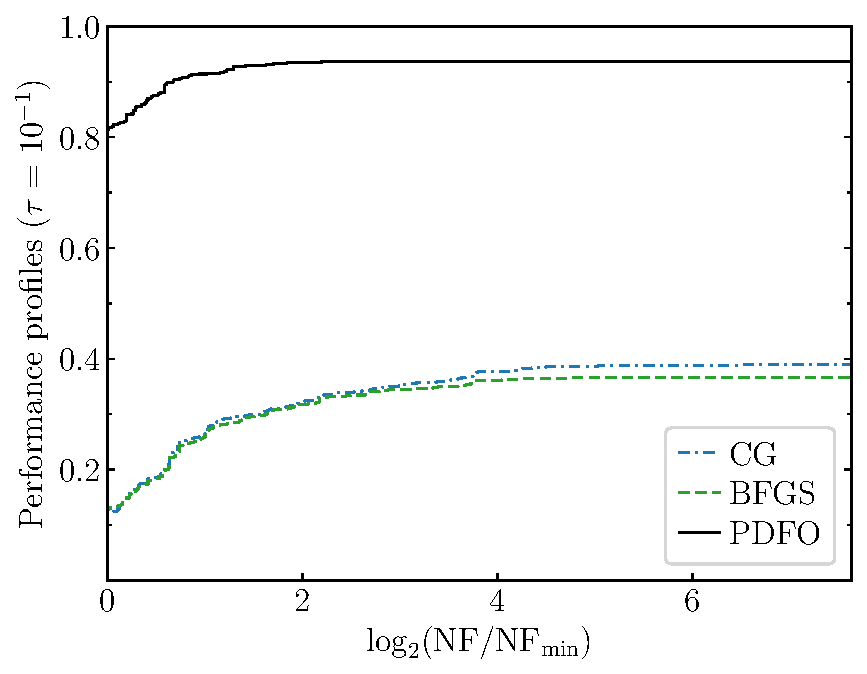
\includegraphics[width=\textwidth]{perf-noisy-bfgs_cg_pdfo-50-8.pdf}
        \caption{Noisy experiment with~$\sigma = 10^{-8}$}
    \end{subfigure}
    \hfill
    \begin{subfigure}{.48\textwidth}
        \centering
        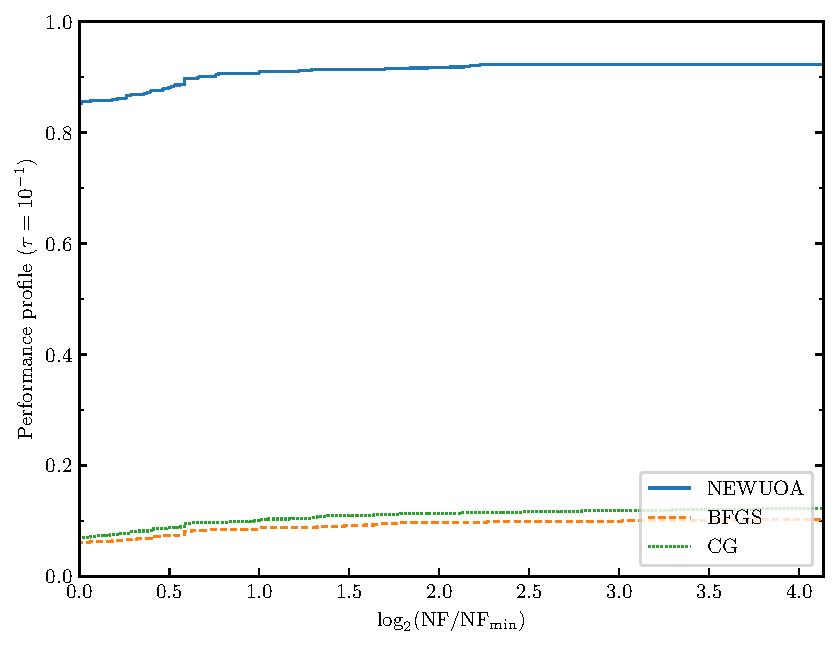
\includegraphics[width=\textwidth]{perf-noisy-bfgs_cg_pdfo-50-6.pdf}
        \caption{Noisy experiment with~$\sigma = 10^{-6}$}
        \label{fig:ppu-fdiff-noisy-6}
    \end{subfigure}
    \caption{Performance profiles of \gls{newuoa}, \gls{bfgs}, and \gls{cg} on problems of dimension at most~$50$}
\end{figure}

Overall, on the noise-free problems, \gls{newuoa} is slightly more reliable than \gls{bfgs} and \gls{cg}.
Moreover, \gls{newuoa} evidently outperforms the two other solvers on noisy problems.
The performances of \gls{bfgs} and \gls{cg} deteriorate significantly when Gaussian noise is imposed as in~\eqref{eq:noisy-obj}, even though the noise level is not high and the convergence tolerance is not demanding.

Note that our results do not contradict the observations in~\cite{Shi_Etal_2022}, where the difference parameter~$h$ is chosen more carefully, according to the noise levels and the smoothness of the problems.
We rather keep the default value provided for the solvers \gls{bfgs} and \gls{cg} by SciPy~\cite{Virtanen_Etal_2020}.
As commented in~\cite{Shi_Etal_2022}, the performance of methods based on finite differences is encouraging when there is no noise, yet much more care is needed when the problems are noisy.
\Gls{newuoa} performs robustly with the noise according to this experiment, which agrees with the observations in~\cite{Shi_Etal_2022}.

We also mention that no conclusive comparison can be made between \gls{bfgs} and \gls{cg} according to Figures~\ref{fig:ppu-fdiff-plain}--\ref{fig:ppu-fdiff-noisy-6}.
In fact, as pointed out in~\cite{Gould_Scott_2016}, when there are more than two solvers to compare, performance profiles have limitations when ranking the solvers, except for the one that outperforms the others (if any), such as \gls{newuoa} in Figures~\ref{fig:ppu-fdiff-plain}--\ref{fig:ppu-fdiff-noisy-6}.

\subsection{Comparison on the CUTEst library}

We now compare the performances of the Powell's \gls{dfo} methods for solving unconstrained problems.
To that end, we first repeat the previously described noise-free experiment.
Performance profiles on unconstrained problems of dimensions at most~$10$ and~$50$ are provided respectively in Figures~\ref{fig:ppu-10} and~\ref{fig:ppu-50}.
According to Figure~\ref{fig:ppu-10}, \gls{uobyqa} performs better than all the other solvers on small problems.
This can be explained by the fact that it uses quadratic models obtained by fully-determined interpolation.
However, we excluded \gls{uobyqa} from the second experiment, because the execution time was excessively long on problems with moderately high dimensions, due to the fully-determined interpolation that it does.
Moreover, \gls{cobyla} is always outperformed by all other solvers.
This is because it uses only linear models to approximate the objective and constraint functions of the problems, which are not as precise as the quadratic models employed by other solvers.

\begin{figure}[ht]
    \begin{subfigure}{.48\textwidth}
        \centering
        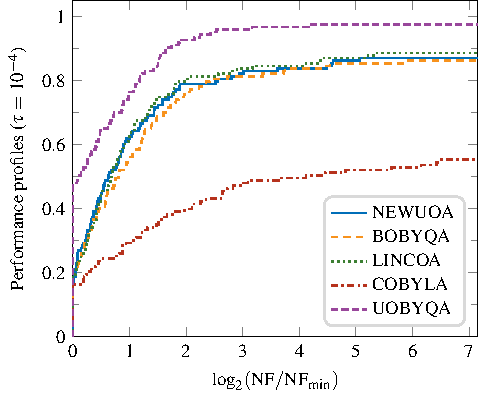
\includegraphics[width=\textwidth]{perf-plain-pdfo-10.pdf}
        \caption{Dimension at most~$10$.}
        \label{fig:ppu-10}
    \end{subfigure}
    \hfill
    \begin{subfigure}{.48\textwidth}
        \centering
        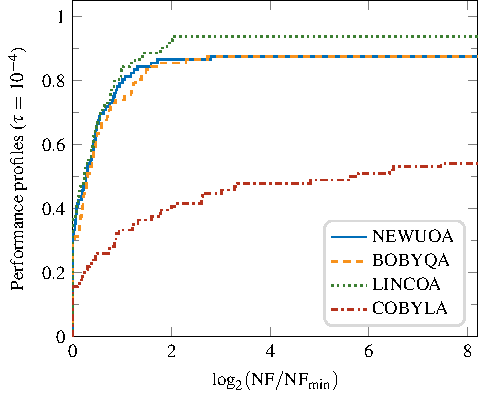
\includegraphics[width=\textwidth]{perf-plain-pdfo-50.pdf}
        \caption{Dimension at most~$50$.}
        \label{fig:ppu-50}
    \end{subfigure}
    \caption{Performance profile of Powell's \glsfmtshort{dfo} solvers}
\end{figure}

Consider however the previously detailed noisy experiment, applied to Powell's \gls{dfo} solvers.
Figure~\ref{fig:ppun-50} presents the performance profiles on the same unconstrained problems of dimension at most~$50$ from the CUTEst library as the previous experiment by randomizing the objective functions with~$\sigma = 10^{-2}$.

\begin{figure}[ht]
    \centering
    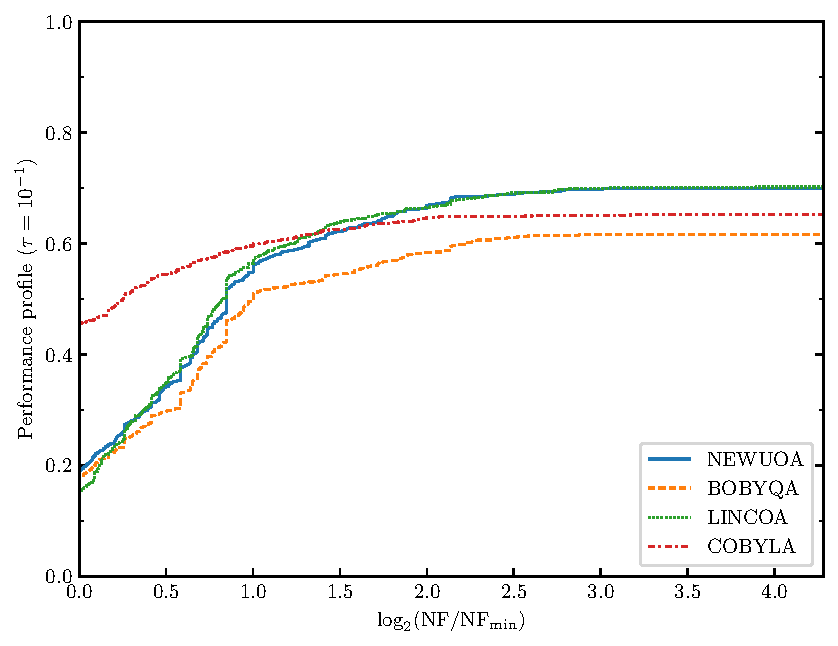
\includegraphics[width=.48\textwidth]{perf-noisy-pdfo-50-2.pdf}
    \caption{Performance profile of Powell's \glsfmtshort{dfo} solvers on noisy problems of dimension at most~$50$}
    \label{fig:ppun-50}
\end{figure}

It is interesting to observe the performance of \gls{cobyla} in this experiment.
Even though it is not particularly designed for such kind of problems and uses the simplest models, we observe that \gls{cobyla} defeats all other solvers on unconstrained problems, for~$\tau = 10^{-1}$.
It seems that the linear models of \gls{cobyla} are more robust to noise, but we have not yet derived a theory for this behavior.

\subsection{An example of hyperparameter tuning problem}

We now consider the more practical problem of the hyperparameter tuning of a \gls{svm}.
The model we consider is a~$C$-SVC~\cite{Chang_Lin_2011} for binary classification problems with an \gls{rbf} kernel, admitting two hyperparameters: a regularization parameter~$C > 0$ and a kernel coefficient~$\gamma > 0$.
We want to compare the performance of \gls{pdfo} with a prominent Bayesian optimization method and \gls{rs}.
To this end, we use the Python package \texttt{hyperopt}~\cite{Bergstra_Yamins_Cox_2013} for solving the optimization problems, which provides both \gls{tpe} and \gls{rs} methods.
Our experiments are based on binary classifications problems from the LIBSVM datasets\footnote{\url{https://www.csie.ntu.edu.tw/~cjlin/libsvmtools/datasets/}.}.
A description of the datasets employed is provided in Table~\ref{tab:htdata}.

\begin{table}[ht]
    \caption{Considered LIBSVM dataset descriptions}
    \label{tab:htdata}
    \centering
    \begin{tabular}{cS[table-format=2]S[table-format=5]}
        \toprule
        Dataset~$\mathcal{P}$   & {Dimension}   & {Dataset size}\\
        \midrule
        splice                  & 60            & 1000\\
        svmguide1               & 4             & 3088\\
        ijcnn1                  & 22            & 49990\\
        \bottomrule
    \end{tabular}
\end{table}

A dataset~$\mathcal{P}$ is formed of two parts: a training dataset~$\mathcal{L}$ and a testing dataset~$\mathcal{T}$, with~$\mathcal{P} = \mathcal{L} \sqcup \mathcal{T}$.

The problem we consider is as follows.
We want to maximize the~$5$-fold \gls{auc} validation score of the \gls{svm} trained on~$\mathcal{L}$ with respect to the hyperparameters~$C$ and~$\gamma$.
The \gls{auc} score, a real number in~$[0, 1]$, measures the area underneath the \gls{roc} curve, a graph representing the performance of a binary classification model.
This curve plots the true positive classification rate with respect to the false positive classification rate at different classification thresholds.
The~$5$-fold \gls{auc} validation score corresponds to the following.
The set~$\mathcal{L}$ is split into~$5$ folds, and the model is trained~$5$ times, on each union of~$4$ distinct folds.
After each training, the \gls{auc} score is calculated on the remaining fold, which was not involved in the training process, giving rise to~$5$ \gls{auc} scores, the average of which corresponds to the~$5$-fold \gls{auc} validation score.

The numerical results for this experiment are provided in Tables~\ref{tab:splice}--\ref{tab:ijcnn1}.
The \gls{auc} scores and accuracies presented in the tables correspond to the ones computed on~$\mathcal{T}$ using an \gls{svm} trained on~$\mathcal{L}$, with the tuned parameters~$C$ and~$\gamma$.

In terms of \gls{auc} score and accuracy, we observe that \gls{pdfo} achieved a clearly better result than \gls{tpe} and \gls{rs} on the ``splice'' dataset, and they all attain comparable results on all the other datasets.
However, \gls{pdfo} always uses much less function evaluations, and hence, much less computation time.
The difference in the computation time is particularly visible on the dataset ``ijcnn1'' in Table~\ref{tab:ijcnn1}, as the size of this dataset is large, so that each function evaluation takes much time.
In summary, we can conclude that \gls{pdfo} performs better than \gls{tpe} and \gls{rs} on these problems.

\begin{table}[!ht]
    \caption{Hyperparameter tuning problem on the dataset ``splice.''}
    \label{tab:splice}
    \centering
    \begin{tabular}{cSSS[table-format=3]S}
        \toprule
        Solver      & {AUC Score ($10^{-1}$)}   & {Accuracy ($10^{-1}$)}    & {No.\ eval}   & {Exec.\ time (\si{\second})}\\
        \midrule
        \Gls{pdfo}  & 9.27                      & 7.37                      & 33            & 5.11\\
        \Gls{rs}    & 5.00                      & 5.20                      & 100           & 8.23\\
        \Gls{rs}    & 5.00                      & 5.20                      & 200           & 16.15\\
        \Gls{rs}    & 5.00                      & 5.20                      & 300           & 24.73\\
        \Gls{tpe}   & 5.00                      & 5.20                      & 100           & 8.22\\
        \Gls{tpe}   & 5.00                      & 5.20                      & 300           & 23.57\\
        \bottomrule
    \end{tabular}
\end{table}

\begin{table}[!ht]
    \caption{Hyperparameter tuning problem on the dataset ``svmguide1.''}
    \centering
    \begin{tabular}{cS[table-format=3]SSS}
        \toprule
        Solver      & {AUC Score ($10^{-1}$)}   & {Accuracy ($10^{-1}$)}    & {No.\ eval.}  & {Exec.\ time (\si{\second})}\\
        \midrule
        \Gls{pdfo}  & 9.95                      & 9.66                      & 51            & 2.83\\
        \Gls{rs}    & 9.94                      & 9.61                      & 100           & 10.22\\
        \Gls{rs}    & 9.95                      & 9.67                      & 200           & 20.51\\
        \Gls{rs}    & 9.95                      & 9.68                      & 300           & 30.75\\
        \Gls{tpe}   & 9.95                      & 9.65                      & 100           & 8.65\\
        \Gls{tpe}   & 9.95                      & 9.68                      & 300           & 22.38\\
        \bottomrule
    \end{tabular}
\end{table}

\begin{table}[!ht]
    \caption{Hyperparameter tuning problem on the dataset ``ijcnn1.''}
    \label{tab:ijcnn1}
    \centering
    \begin{tabular}{cS[table-format=3]SSS}
        \toprule
        Solver      & {AUC Score ($10^{-1}$)}   & {Accuracy ($10^{-1}$)}    & {No.\ eval.}  & {Exec.\ time (\SI{}[10^3]{\second})}\\
        \midrule
        \Gls{pdfo}  & 9.97                      & 9.80                      & 44            & 2.48\\
        \Gls{rs}    & 9.97                      & 9.82                      & 100           & 3.99\\
        \Gls{rs}    & 9.98                      & 9.77                      & 200           & 7.60\\
        \Gls{rs}    & 9.97                      & 9.77                      & 300           & 11.52\\
        \Gls{tpe}   & 9.98                      & 9.79                      & 100           & 3.42\\
        \Gls{tpe}   & 9.98                      & 9.79                      & 300           & 8.81\\
        \bottomrule
    \end{tabular}
\end{table}
